\irsection{Runing and testing the \icofoam\, module}{RunModule}

Now that the library and driver for the module have been built, run the driver executable in the same manner in which \elmer was run in the example problem discussed in Section 4.3 and 4.4 of the \irfilename{Uniphysics Validation for Development of Multiphysics Coupling in MP-Infra} document (mentioned in \irref{Section}{elmer}). \textbf{Note:} Remember to double check your environment variables. Ensure that the module driver achieves the same results as using the initial \texttt{Elmer} executable. \irref{Figure}{fig:elasticBeam} shows the results of the simulation.
 
\begin{figure}[H]    
\centering
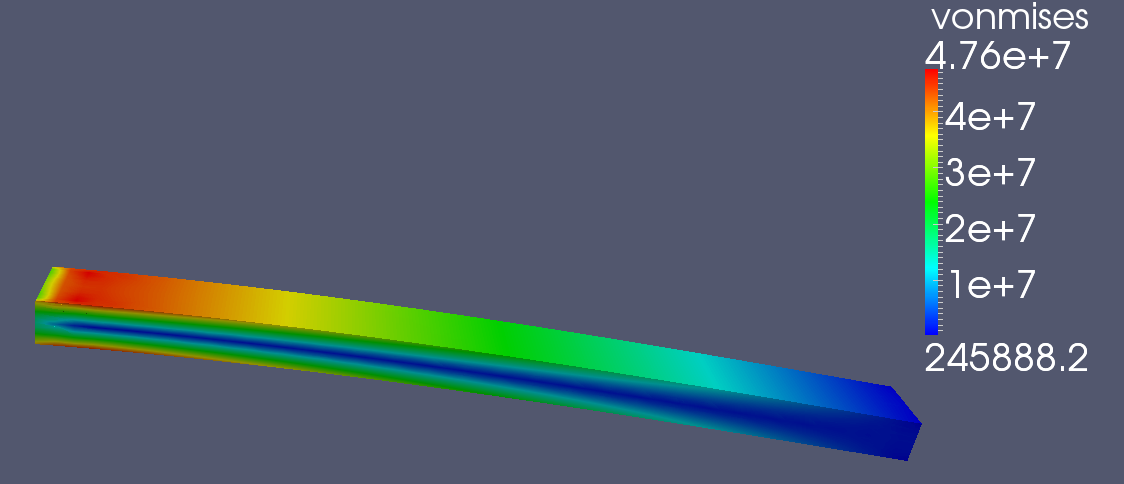
\includegraphics[width=0.85\textwidth]{../Figures/elasticbeam.png}
\caption{Results of elastic beam example run with \software{Elmer IMPACT} module}.
\label{fig:elasticBeam}
\end{figure}
